\chapter{基于密集型自底向上网络的视频片段检索方法}

在本章,我们主要解决视频片段检索任务。具体来说,给定一个查询(如:自然语句或者视频片段)和一段未裁剪的视频序列,模型需要在视频序列中定位出和查询内容相匹配的片段。目前,主流的视频片段检索方法可以分为两大类:(1)自顶向下(Top-down)的方法:它们先将整个视频序列切分为若干候选片段,然后对每个候选片段进行分类和回归。分类主要是计算候选片段与查询的相似度,回归主要是微调片段的位置。(2)自底向上(Bottom-up)的方法:先将视频序列和查询进行特征融合,然后对融合后的特征序列中的每一帧预测其属于视频序列定位边界的概率(起始时刻和终止时刻)。然后这两类方法都各自具有明显的缺点:自顶向下的方法需要人为地预先设定许多切分的规则(如:候选片段的大小、候选片段的数量等)同时定位速度也较慢,而自底向上的方法的性能还低于自顶向上的方法。在本章,我们重点分析了目前的自底向上方法的设计缺陷,提出了一种全新的密集型自底向上框架。我们将位于起始时刻和终止时刻之间的每一帧都看成是正样本,每一个正样本帧都回归一个独特的离定位边界的距离。同时为了更好的适应密集型自底向上的框架,我们还提出了一种基于图结构的特征金字塔网络,来强化目前的骨干网络(backbone)。我们先将多尺度的特征帧映射到同一个语义空间中,然后利用图卷积学习到语义空间中不同特征的内在联系。我们在常用的四个视频片段检索数据集(TACoS~\cite{regneri2013grounding}、Charades-STA~\cite{gao2017tall}、ActivityNet Captions~\cite{krishna2017dense}、Activity VRL~\cite{feng2018video})中验证了我们方法的有效性,我们提出的密集型自底向上网络不仅可以在性能上超过目前所有的方法,同时可以保持和其他自底向上的模型相同的定位速度。


\section{问题描述}

基于查询的视频片段检索是视频场景理解领域一个重要的研究问题。它不仅仅需要准确地把握检索内容的语义信息,同时需要对视频内容有正确的理解。随着大规模视频数据集的出现和视频特征学习的发展,目前主要有两种视频片段检索任务:(1)第一种是基于语句的视频片段检索,即查询内容是一个自然语言描述语句(如图~\ref{ch5:fig:qbvl}(a))。(2)第二种是基于视频片段的视频片段检索,即查询内容是包含一个动作的短视频片段(如图~\ref{ch5:fig:qbvl}(b))。这两种视频片段检索任务拥有同样的目标:在视频序列中定位出两个边界时刻(即起始时刻和终止时刻),使得从起始时刻到终止时刻之间的视频片段内容刚和和查询内容一致。视频片段检索任务也是许多重要的视频应用的技术基础,例如:基于内容的精彩片段检索、行人重识别等。

\begin{figure}[htbp]
    \centering
    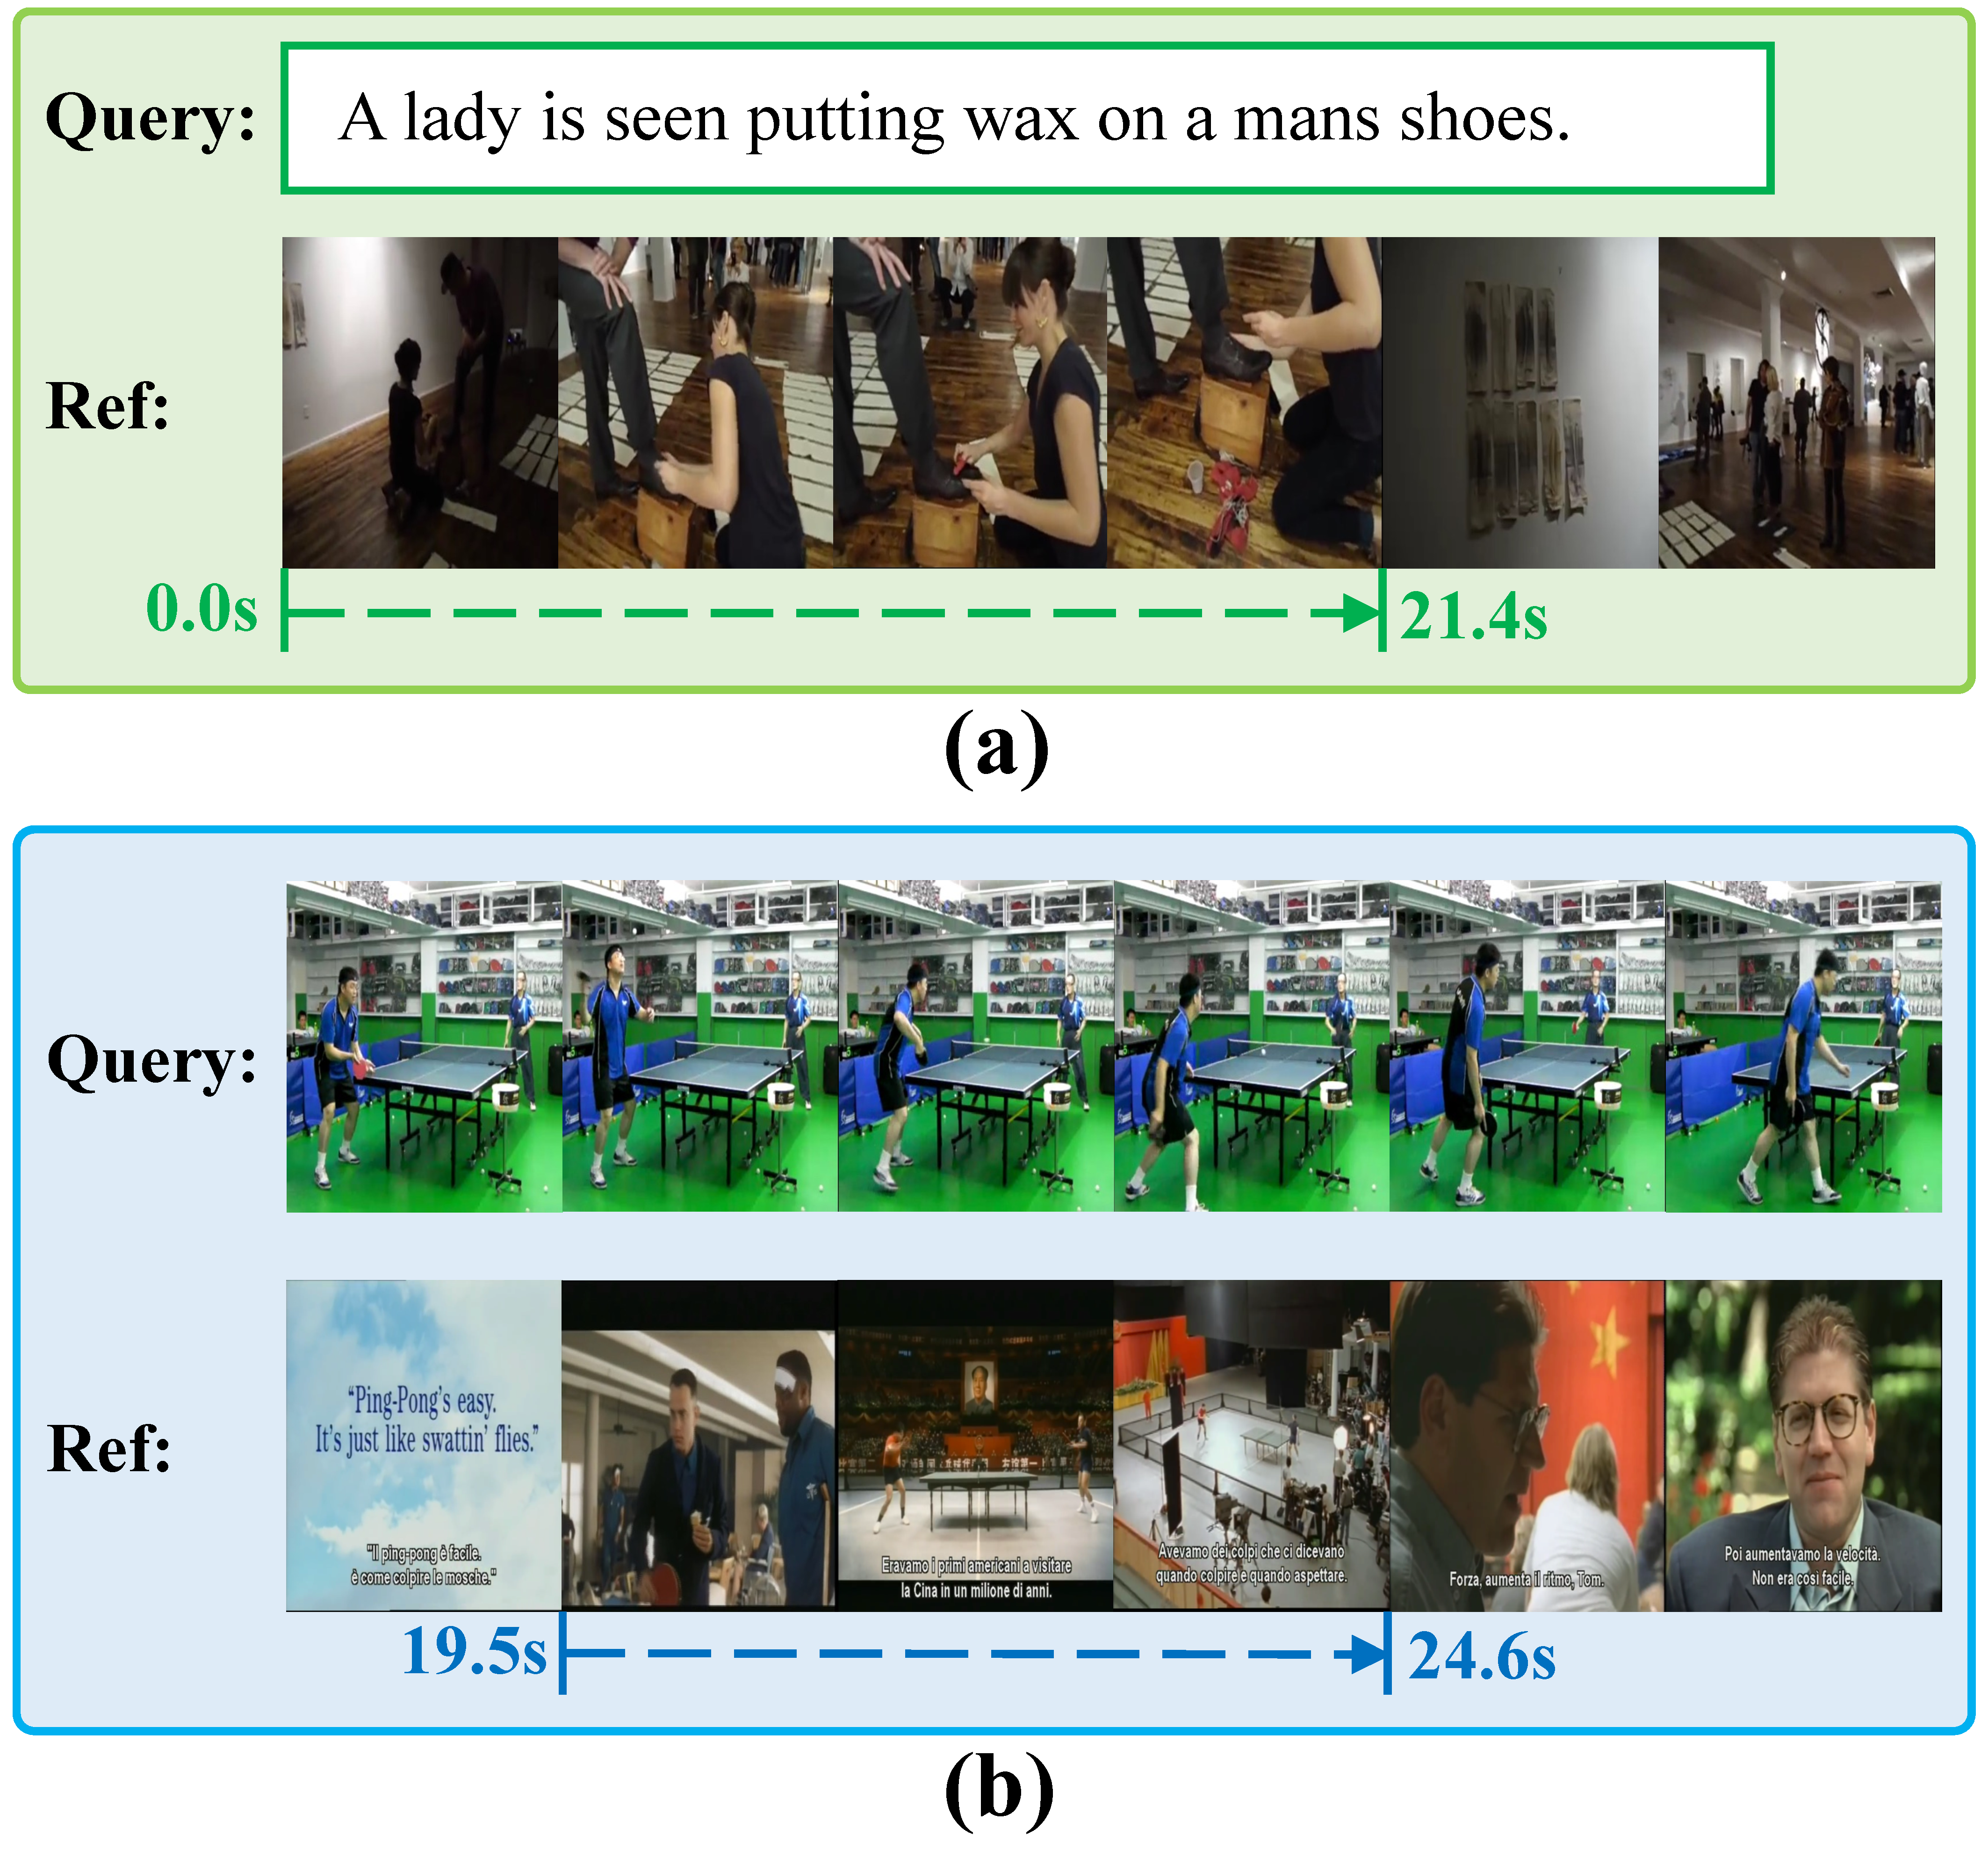
\includegraphics[width=0.7\linewidth]{chapter6/res/qbvl.pdf}
    \caption{两种视频片段检索任务}
    \label{ch5:fig:qbvl}
\end{figure}

到目前为止,绝大多数的视频片段检索方法都是\textbf{自顶向下}的方法:

\section{密集型自底向上框架}


\section{基于图结构的特征金字塔网络}


\section{实验设置与性能对比}

\subsection{视频片段检索数据集}

\noindent\textbf{\kaishu{基于语句的视频片段检索}}:我们在以下三个数据集上进行评估:

\noindent\textbf{TACoS}~\cite{regneri2013grounding}:它一共包含127个视频和17344个文本与视频序列对(样本)。我们参考现有的标准数据集划分~\cite{gao2017tall},将其中50\%的样本作为训练集,25\%的样本作为验证集,25\%的样本作为测试集。每个样本中视频的平均长度为5分钟。


\noindent\textbf{Charades-STA}~\cite{gao2017tall}:它一共包含12408个文本与视频序列对作为训练集,3720个文本与视频序列对作为测试集。每个样本中视频的平均长度为30秒。


\noindent\textbf{ActivityNet Captions}~\cite{krishna2017dense}:它是目前为止最大、最丰富的数据集,一共包含19209个视频。我们参考现有的工作~\cite{yuan2019find}, 使用37421个文本与视频序列作为训练集,17505个文本与视频序列作为测试集。每个样本中视频的平均长度为2分钟。


\noindent\textbf{\kaishu{基于视频的视频片段检索}}:我们在以下数据集上进行评估:

\noindent\textbf{ActivityNet-VRL}~\cite{feng2018video}:它是目前唯一公开发布的数据集。它对动作识别数据集ActivityNet~\cite{caba2015activitynet}共200个类别的视频进行了重组,其中任意选取160个类别对应的视频作为训练集,20个类别对应的视频作为验证集,以及剩余20个类别对应的视频作为测试集。这种零样本式的数据集划分能够评估模型的泛化能力。在训练阶段,查询视频和引用视频是随机选取的。在测试阶段,查询视频和引用视频是固定的。

\subsection{评价指标}


\noindent\textbf{\kaishu{基于语句的视频片段检索}}:我们参考现有工作,使用下列两种通用的评价指标:

\noindent\textbf{R@N, IoU@$\theta$}:在测试集中,每个样本预测分数最高的n个的结果重叠度(Intersection-over-Union,IoU)大于$\theta$的百分比。由于自底向上框架的特性,我们仅考虑$N=1$。

\noindent\textbf{mIoU}:测试集中所有测试样本的平均的重叠度。


\noindent\textbf{\kaishu{基于视频的视频片段检索}}:我们使用以下评价指标:

\noindent\textbf{mAP@1}:在不同阈值下最高预测结果的平均精度均值(mAP)。

\section{本章小结}

